\begin{figure*}[htbp]
\centering
\vspace{-2mm}
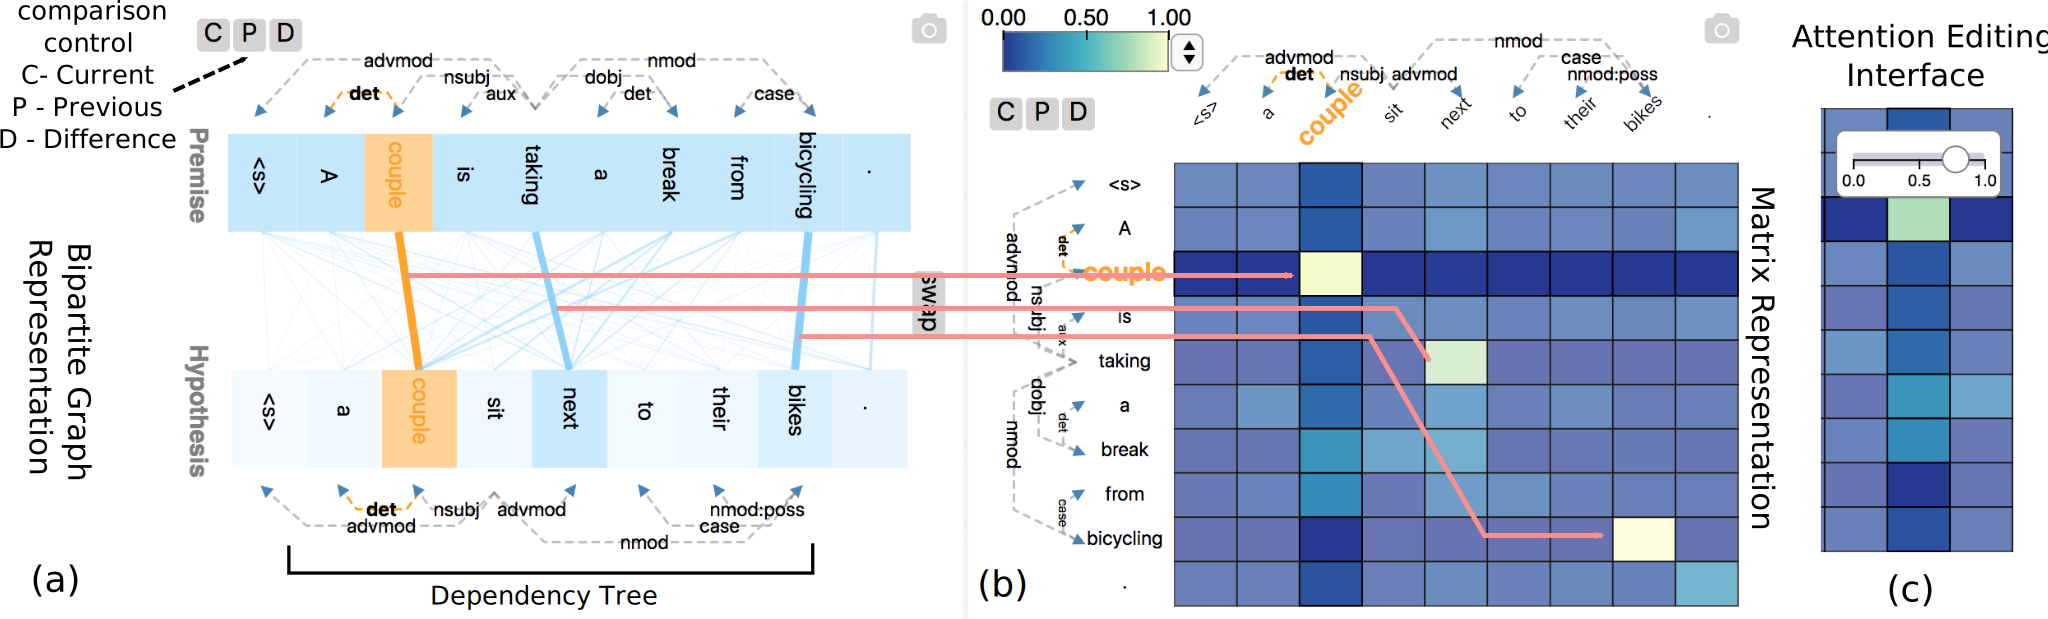
\includegraphics[width=1.0\linewidth]{attentionView}
\vspace{-6mm}
\caption{
Attention visualization. In the graph attention view (a), a bipartite graph encoding is adopted, in which the edge thickness corresponds to the attention value. In the matrix attention view (b), the $i^{th}$ row corresponds to the probability of words in hypotheses align to the $i^{th}$ word in the premise.
The user can alter the attention values via the pop up interface illustrated in (c).
}
\label{fig:attentionVis}
\end{figure*}

\subsection{Attention View}
\label{sec:attention}
\shusen{How to fit dependency into the task, what is the motivation}
As discussed in Section~\ref{sec:attention}, the attention is the only intermediate layer in the network that provide interpretable information for domain expert to infer the inner mechanisms of the model.
%
Intuitively, the attention captures the alignment of words between input sentences. In the NLI model examined in this work, the attention is represented as a matrix, in which the $i^{th}$ row corresponds to the probability of words in hypotheses align to the $i^{th}$ word in the premise.
% The

As illustrated in Fig.~\ref{fig:attentionVis}, we employ too visual encoding for attention. In the graph attention view (a), a bipartite graph encoding is adopted, in which the edge thickness corresponds to the attention value. Such a view is good for highlight the most dominate alignments. However, if many attention values are high, the edges may become cluttered lead to less effective visualization. In addition, if the sentence structure different between premise and hypothesis is drastically different, we are likely to see the prominent edges cross each other, which can also lead to confusing visual patterns. The matrix attention view (b), despite being more verbose and less efficient in highlighting the dominate alignment, do not have similar shortcomings. Together them complement each other and provide the same information from different perspective. As illustrated by the pink arrow line, we can see how the same attention value is visualization in both the grpah and the matrix view.
To help the user recongnize the correspondence during the exploration, we enable the linkage between highlight actions in both view.

To full address the \emph{T2}, we also include the attention editing functionality. The attention matrix view is the most suitable place conduct the edit, since it provide a direction mapping of attention value.
As we can see in Fig.~\ref{fig:attentionVis}(c), when the cell of the matrix is clicked, a sider will pop up to allow user customize the attention value (as the user edit the value, each row will be automatically normalized).
%allow the user to view all the values clearly.


%\subsubsection{Attention visualization challenges}
% \begin{itemize}
% 	\item Why we need two different visual encoding to visualize attention? bipartite visualization more easier to highlight the
% 	\item long sentence, collapse
% 	\item quickly compare the alignment information with the sentence's linguistic structure.
% \end{itemize}


% \subsection{Interpret Attention Via Model Perturbation}
